%% This is an abbreviated template from http://www.sigplan.org/Resources/Author/.

\documentclass[acmsmall,review,authorversion]{acmart}
\acmDOI{}
\acmJournal{FACMP}
\acmVolume{CSCI 5535}
\acmNumber{Spring 2020}
\usepackage{graphicx}
\usepackage{amssymb}
\usepackage{mathtools}
\usepackage{amsmath}
\usepackage[linesnumbered,ruled]{algorithm2e}
% \graphicspath{ {./assets/} }

\begin{document}

%%
%% The "title" command has an optional parameter,
%% allowing the author to define a "short title" to be used in page headers.
\title{A Framework for Formal Verification to Correct Actions in Reinforcement Learning}

%%
%% The "author" command and its associated commands are used to define
%% the authors and their affiliations.
%% Of note is the shared affiliation of the first two authors, and the
%% "authornote" and "authornotemark" commands
%% used to denote shared contribution to the research.
\author{Ethan Hobbs}
\email{ethan.hobbs@colorado.edu}
\author{Vikas Nataraja}
\email{viha4393@colorado.edu}
\affiliation{%
  \institution{University of Colorado Boulder}
}


%%
%% The abstract is a short summary of the work to be presented in the
%% article.

\begin{abstract}
In reinforcement learning, proving the possibility of a safe state is inherently difficult due to the range of methods available to find a new safe state. One of the most common options for finding a new state when the agent reaches an unsafe one is reverting to an initial state. In many cases, these methods are inefficient or might not actually produce a safe state transition. In this paper, we propose a new method for verifying an agent's policy for transitioning out of an unsafe state in the immediate future by using backtracking to guarantee safe state transition.
\end{abstract}

%%
%% This command processes the author and affiliation and title
%% information and builds the first part of the formatted document.
\maketitle

\section{Introduction}
Reinforcement Learning (RL) has gained immense momentum in recent years particularly in the field of robotics where tasks are repetitive and RL can make an instant impact. This is because the agent can learn a policy that maximizes the reward function much quicker in repetitive tasks because the reward environment is denser and guarantees near-continuous rewards for every action that the agent takes. With RL gaining popularity, verification of such systems is an active area of research in Computer Science. The core problem of any software verification is to verify that a given system satisfies its specification. A conventional way to verify software in general is to establish safety rules before the agent is deployed in the environment which requires extensive data \cite{gopinath:2017}. It is not always possible to predict the states or the changes in the environment beforehand particularly if it is dynamically changing. Another common approach that is more widely deployed in Machine Learning is for the system itself to verify its own progress \cite{zhu:2019,sun:2019}. While it is difficult to characterize such a verification, it affords better safety which is essential in RL (and relational verification of RL). Formal state verification then becomes essential so that the agent can monitor its progress by checking the validity of states. We propose \emph{backtracking} through past states to avoid transitioning to an invalid or unsafe state similar to the method proposed by Goyal et al. \cite{DBLP:journals/corr/abs-1804-00379}

\section{Overview}
In our implementation of the system, we synthesize a deterministic program that approximates the neural network policy developed by the reinforcement learning algorithm. We then verify the deterministic version of the program and use it to shield the actual neural policy from entering into an unsafe state. In the verification, we look at a transition from state $a$ to state $b$ dependent on whether state $b$ is ``safe.'' Safe in this context means that the state is reachable by the reinforcement learning system and that it will not violate the failure conditions set out in the reinforcement system. While the verification process gives us a good idea on what is a safe state, it will not guarantee it since the synthesized program is an approximation. We then have to perform a second shielding step at run-time to prevent any edge cases. This method described above has previously been explored in Zhu et al. where for the safety verification algorithm, the diameter of the state space is reduced by a factor of $0.5$ when a counterexample is found \cite{zhu:2019}. Since reinforcement learning systems like a robotic arm are physical, it would be desirable to create a more representational state space transformation rather than the simple reduction. If this is done, an operation like restoring to the previous safe state could be performed if a counterexample is found in the transitions of the current state.

Consider a cartpole system which is an extension of the classical inverted pendulum problem. A pole is attached by an un-actuated joint to a cart, which moves along a frictionless track. The system is controlled by applying a discrete force measure to the cart. The pendulum starts upright, and the goal is to prevent it from falling over. Assuming a \emph{fully observable} system, the observation space then becomes the cart velocity, cart position, pole angle and the pole velocity at the tip. Using these parameters, again, under the assumption that these are fully observable, we can describe the entire system. The action space is discrete and binary - moving the cart to the left or the right but not both. Details about the dynamics and specifics of the cartpole environment are explained in Section 6.

\section{Reinforcement Learning Background and Terminology}
This section will detail some basic concepts in reinforcement learning such as Q-learning, policies, rewards and other common terminology used in reinforcement learning that will be used in subsequent sections.

\subsection{Q-learning}
Q-learning was first introduced in 1992 by Watkins et al. as a way for an RL agent to learn an optimal policy in a Markov Decision Process (MDP) \cite{Watkins92q-learning}. Since then, it has gained immense popularity and is one of the most common ways of learning a policy. It uses a \emph{Q} function to learn a policy for a state-action pair. At the start of the episode or session, all Q values are initialized with zeros and for each state, every action possible at that state has an associated reward for taking that action, keeping in mind that rewards can be negative as well to indicate that the agent chose the "wrong" action and learned a sub-optimal policy. and are cumulatively used to learn a better policy at each timestep depending on the reward. After every action is taken and an outcome is observed, the \emph{Q value} is updated. At each timestep, the maximum expected future reward is balanced against optimizing current state-action policy by using $\gamma$ which is called the \emph{discount factor}.

\[\underbrace{\text{New}Q(s,a)}_{\scriptstyle\text{New  Q-Value}}=Q(s,a)+\mkern-34mu\underset{\text{Learning Rate}}{\underset{\Bigl|}{\alpha}}\mkern-30mu[\underbrace{R(s,a)}_{\scriptstyle\text{Reward}}+\mkern-30mu\underset{\text{Discount factor}}{\underset{\Biggl|}{\gamma}}\mkern-75mu\overbrace{\max Q'(s',a')}^{\scriptstyle\substack{\text{Maximum predicted reward, given} \\ \text{new state and all possible actions}}}\mkern-45mu-Q(s,a)]\]

\subsection{Deep Q-learning}
Deep Q-learning is an extension of the Q-learning scheme and improves upon it by speeding up the learning process using deep neural networks and reduces memory consumption. Classical Q-learning works well for environments with a small number of states and actions because the Q-table can be easily built. But it cannot handle computation for environments having hundreds or thousands of states and actions because saving the Q-table in memory is simply unrealistic. Deep Q-learning overcomes this problem by approximating the Q-value using neural networks trained as a regression problem and evaluated under appropriate loss functions like mean squared error. For each state, it approximates the actions and chooses the \emph{best} action for that state and records progress in the experience replay buffer. In our proposed method, we employ a deep Q-network to solve the evaluation scenario, more details are available in Section 5.

    \begin{figure}[ht]
        \centering
        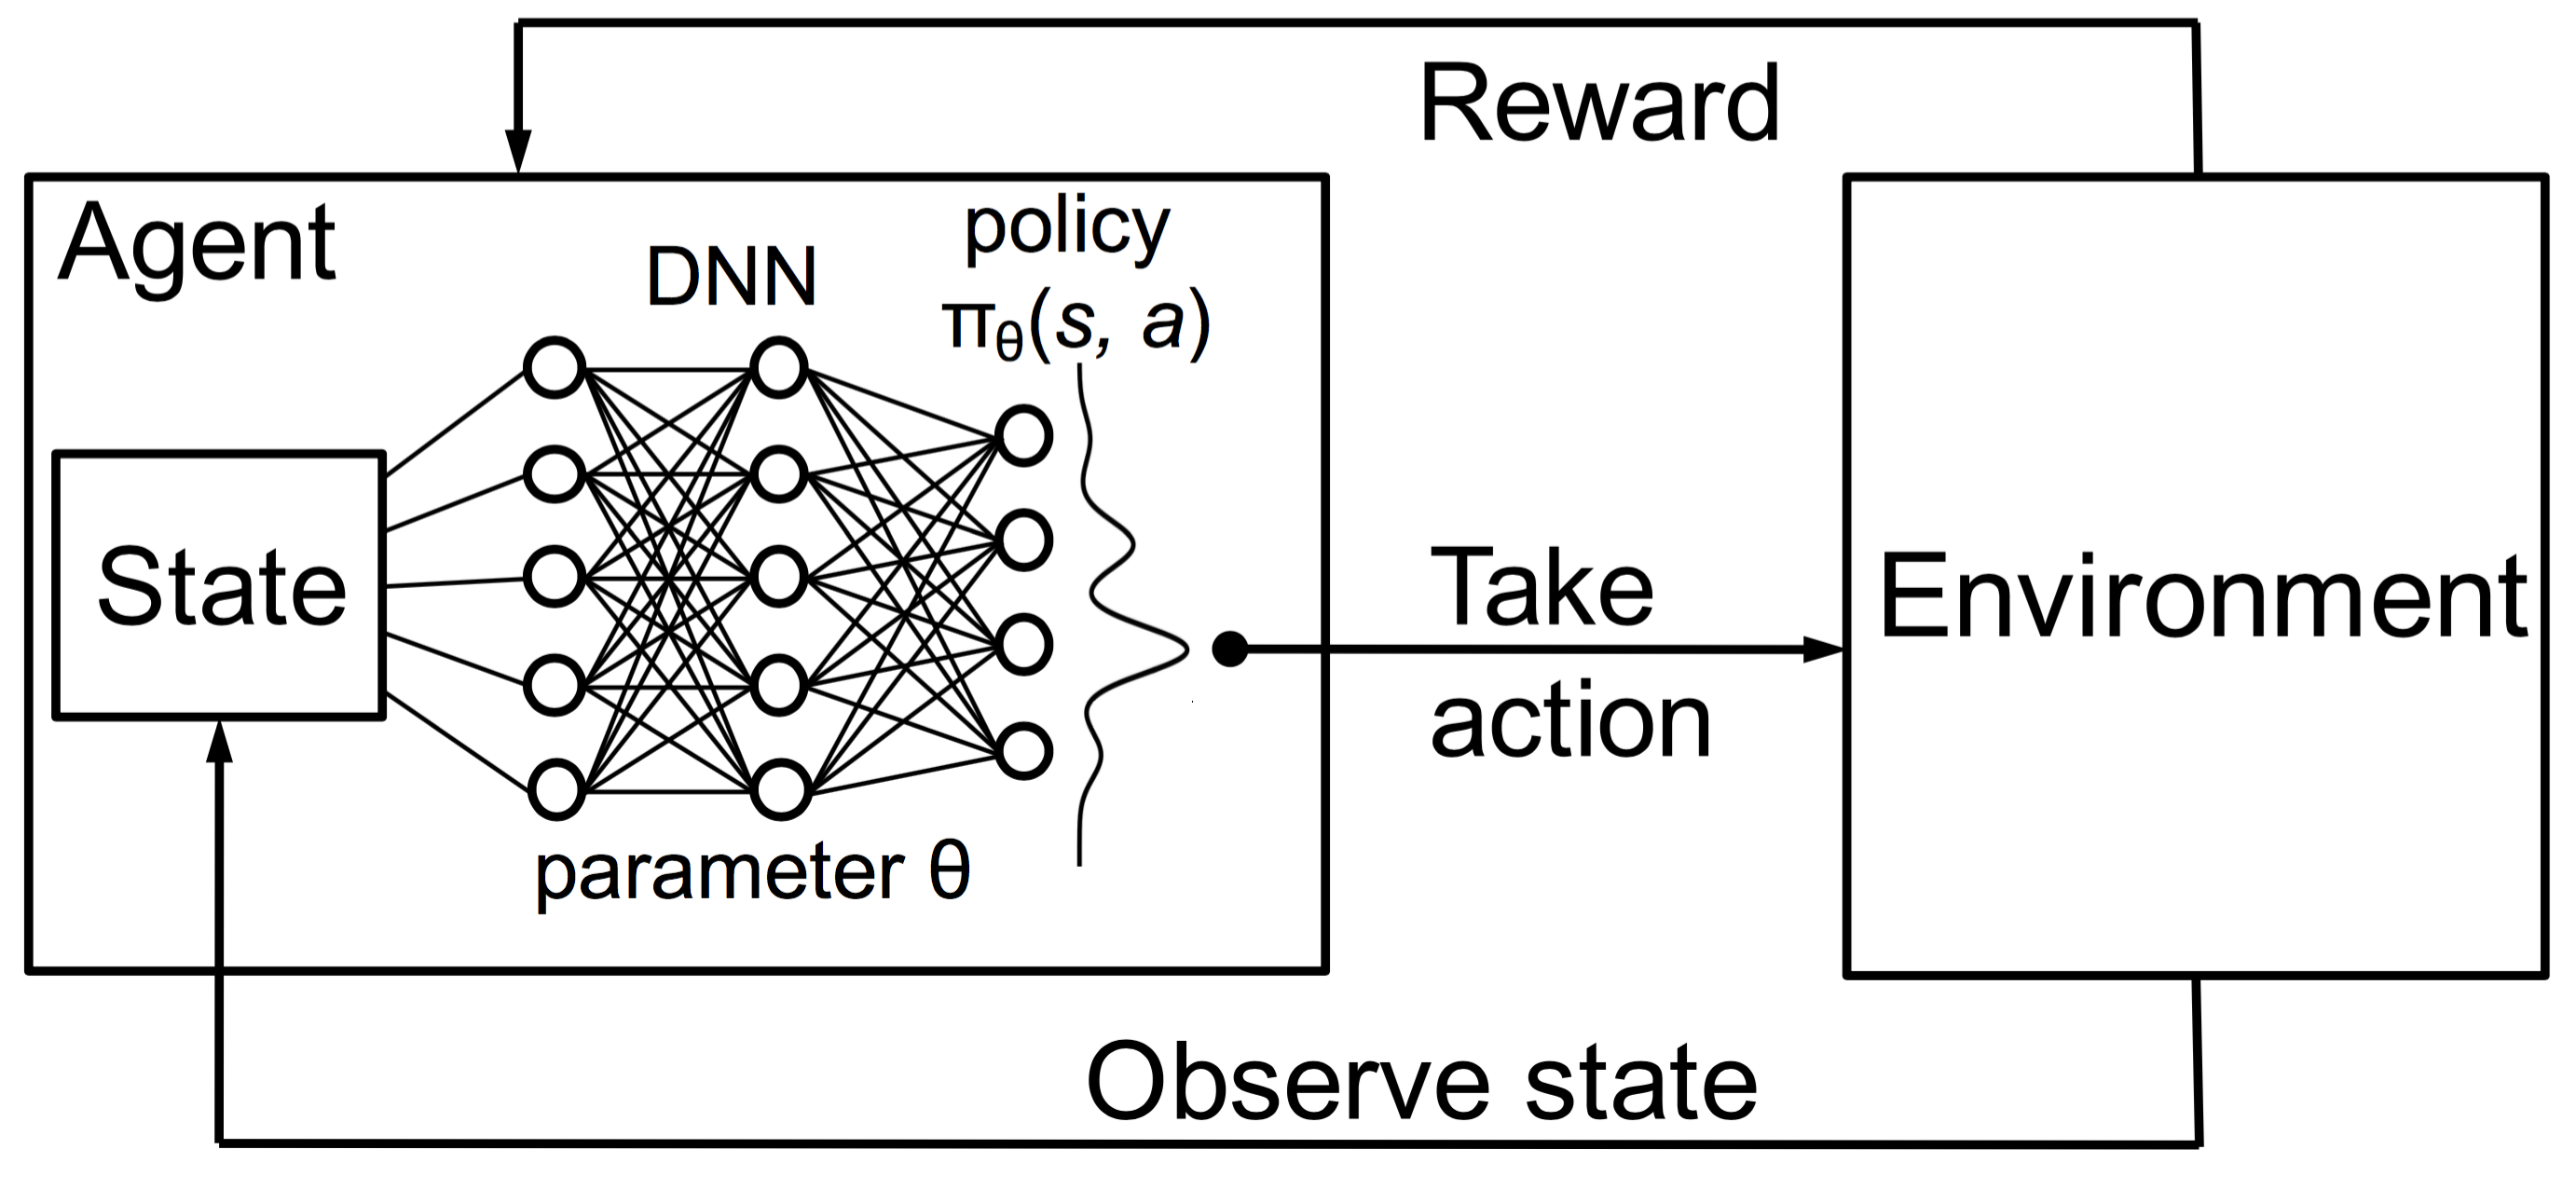
\includegraphics[width=0.65\textwidth]{assets/dqn.png}
        \caption{Schematic representation of a Deep Q-network}
        \label{fig:DQ_schem}
    \end{figure}

\subsection{Replay Buffer}
The replay buffer, also called experience replay, is a technique used to allow the agent to learn from previous experiences and thereby improving learning by making better informed decisions about the action to be taken at a state. The experiences are stored in a buffer with a preset memory size and the size of the memory can affect the speed of computation. Liu et al. explored the effects of changing memory sizes and found that too much or too little memory slow down the learning process \cite{DBLP:journals/corr/abs-1710-06574}. In our proposed work, we use the replay buffer to traverse through the history of saved states to find a safe state. The states in the buffer are guaranteed to be safe because the agent has continued learning and has updated its policies after passing those states.


% \section{(Contribution 1)}

\section{Technical Contributions}
\subsection{From Policy to Deterministic Program}
This section is not completed yet and will be updated in the final draft.
\subsection{Verification Process}
With the method for synthesizing the deterministic policy, we now can verify the program. We chose to do a runtime verification method that will be assessed at each action taken by the agent. We developed an algorithm (seen in Algorithm \ref{Alg:verif}) that shows how this is possible. The first step is to synthesize a deterministic program with the method described in the previous subsection. With this deterministic approximation, we then can project forward in time $n$ number of steps in the future. In general we want this $n$ to be small for performance and speed purposes. This step allows us to see in the future what possible valid states there are as defined by the reinforcement learning scenario. If there is at least one valid state reachable from the current state in $n$ steps we proceed with the reinforcement learning and take the action determined by the policy. Otherwise if there are no valid states, we do not want to advance further down this path. Since we have discrete states, we chose to backtrack to the a previous safe state from $m$ steps ago and reclassify the current state as unsafe effectively cutting off the branch of the state network.
\begin{algorithm}[ht]
    synthesize the deterministic program\\
    Project forward $n$-steps\\
    Check the validity of possible states \\
    \eIf{valid states $\geq 1$}
      {
        proceed with reinforcement learning
      }
      {
        return to the state $m$ states ago
      }
 \caption{Verification Algorithm}
 \label{Alg:verif}
\end{algorithm}{}
\section{Empirical Evaluation}
This section details our evaluation procedure and offers insight into different scenarios in RL Specifically we discuss the dynamics of the system including reward and state actions.

Our proposed method was implemented in OpenAI Gym's cartpole environment \cite{DBLP:journals/corr/BrockmanCPSSTZ16}. Specifically, we implemented our model in the cartpole scenario, an extension of the inverted pendulum environment. The goal is to balance the cartpole without it falling over. The environment offers a force unit of +1 and -1 using which the pole can be balanced. For every timestep that the pole doesn't fall over, a +1 reward is provided. Note that this can be changed to suit different positive discrete value. The state space, which is now fully observable because of dense rewards, becomes our observation space which can be seen in Table 1. The agent's episode ends when the pole is more than 15 degrees from vertical, or the cart moves more than 2.4 units from the center after which the subsequent episode starts. 

\begin{table}[hbt]
\begin{tabular}{|l|l|l|l|}
\hline
Num & Observation & Min & Max  \\ \hline
0 & Cart Position & -2.4 & 2.4 \\ \hline
1   & Cart Velocity & $-\infty$ & $\infty$ \\ \hline
2   & Pole Angle & $\sim -41.8^\circ$ & $\sim41.8^\circ$ \\ \hline
3   & Pole Velocity at Tip & $-\infty$ & $\infty$ \\ \hline
\end{tabular} 
\caption{Observation Space constraints for Cartpole environment}
\label{tab:cartpole}
\end{table}
% the second half of this paragraph probably needs to be moved to an earlier section 
To compare against, we chose the baseline to be a deep Q-network with 4 fully-connected or dense layers, each with non-linear ReLU (Rectified Linear Action Unit) except for the final layer that uses a linear activation because the output is a discrete value to be regressed over. The code is available on Github (link to Github goes here). Our proposed model implements a deep Q-network with state backtracking (not to be confused with neural network back propagation which uses gradients and derivatives to learn). To achieve this, we leveraged the agent's state history which is already cached in the replay buffer (also called experience replay and memory replay). This also enables the agent to learn from off-policy experiences to better judge future state-action pairs. We expect our model will take more time to solve the cartpole environment because of the aforementioned backtracking. However, by sacrificing speed and going for a temporarily sub-optimal policy, we gain the guarantee that the agent never ends up in an unsafe or invalid state.

\section{Related Work}
In recent years, significant work has gone into verification of reinforcement learning and more specifically, the verification of states. A two-pronged system was implemented by Zhu et al. where the concept of safety and safety verification were both baked into the synthesis of a deterministic program with an inductive invariant alongside the neural policy \cite{zhu:2019}. However, when an invalid or incorrect state is observed, the agent reverts to one of initial safe states. In our approach, the agent back propagates to an already traversed safe state.
A similar formal verification approach was taken by Sun et al.  but to verify the actions of an autonomous robot by constructing a finite state abstraction and performing reachability analysis over the search space \cite{sun:2019}. However, if the initial set of safe states are not within a certain limit, there is a high risk of state space explosion.At the same time, it does not apply to unbounded states and does not capture the relationships between the state variables. These shortcomings are bypassed in our approach because we use the existing state space to find a safe state. Singh et al. introduced a method to certify deep neural networks by using a novel abstract interpreter which relies on a combination of floating-point polyhedra and activation functions such as ReLU (Rectified Linear Unit) and the sigmoid function \cite{singh:2019}. While this approach works to prevent exploding gradients during training, it works by transforming activation functions which inherently means that the neural network, in its current form, cannot be made robust to deeper architectures. In our proposed framework, we eliminate the need for changing activation functions by solving for state space. Chen et al. focused on relational verification represented as a Markov Decision Process (MDP) solvable via reinforcement learning \cite{chen:2019}. The problem with MDPs is that high-dimensional state spaces are not solvable. In our proposed method, we aim to use the existing policy to find a safe state which does not expand the dimensionality.



\section{Conclusion}

\section{Future Work}
%%
%% The acknowledgments section is defined using the "acks" environment
%% (and NOT an unnumbered section). This ensures the proper
%% identification of the section in the article metadata, and the
%% consistent spelling of the heading.
\begin{acks}
TBD
\end{acks}

%%
%% The next two lines define the bibliography style to be used, and
%% the bibliography file.
\bibliographystyle{ACM-Reference-Format}
\bibliography{references}
\end{document}